\anonsection{Цель лабораторной работы}
Лабораторная работа №3 выполняется на основе лабораторной работы №2.
Ее цель заключается в отработке навыков использования программы Microsoft Project для оптимизации временных и финансовых показателей
проекта.

Команда разработчиков из 16 человек занимается созданием карты города на основе собственного модуля отображения. 
Проект должен быть завершен в течение 6 месяцев. Бюджет проекта: 50 000 рублей

\newpage
\anonsection{Задание 1}
В этом задании требуется выравнить загрузку ресурсов в проекте.

По итогам прошлой лабораторной работы выяснилось, что несколько ресурсов перегружены:
\begin{itemize}
	\item \textbf{Системный аналитик} вынужден одновременно выполнять две задачи – «Анализ и построение структуры базы объектов» и «Анализ и проектирование ядра».
	\item \textbf{Художник-дизайнер} должен одновременно выполнять две задачи – «Разработка дизайна руководства» и «Разработка дизайна сайта».
	\item \textbf{Технический писатель} вынужден одновременно выполнять две задачи: «Создание справочной системы» и «Написание руководства пользователя»
\end{itemize}

Для ликвидации перегрузки этих ресурсов использовалось \textit{Автоматическое выравнивание загрузки ресурсов}.
Этот пункт можно выбрать в меню \textit{Ресурсы}.

\newpage
На рисунке 1 представлены параметры, с которыми использовалось выравнивание:
\FloatBarrier
\begin{figure}[h]	
	\begin{center}
		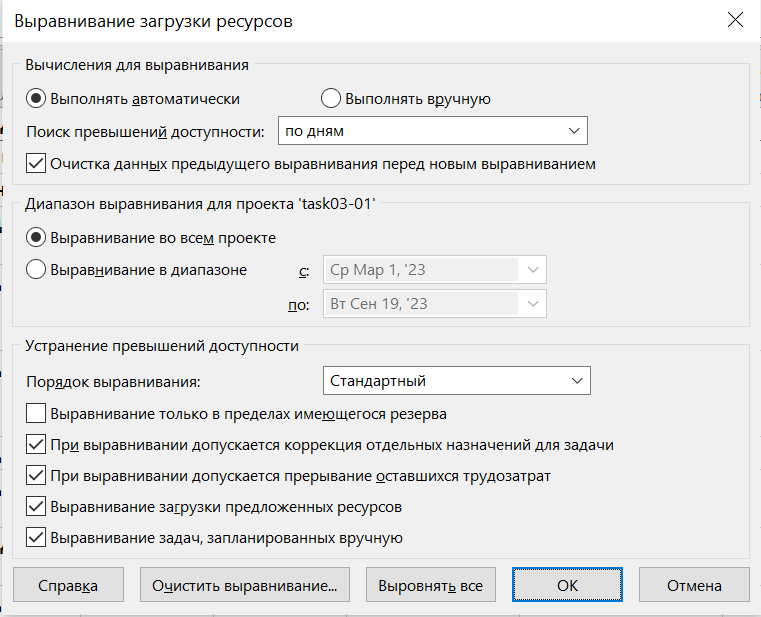
\includegraphics[width=\linewidth, height=9cm]{inc/vyr.png}
	\end{center}
	\captionsetup{justification=centering}
	\caption{Выравнивание загрузки ресурсов}
\end{figure}
\FloatBarrier 

Поиск превышения доступности выбран по дням, так как для Художника-Дизайнера и Технического писателя повышенная загрузка наблюдается в течение лишь нескольких дней, а сам проект пока спроектирован так, что уже есть отставание на неделю -- терять ещё одну неделю нельзя.

В результате перезагруженность ресурсов была ликвидирована.
На рисунке 2 изображена текущая загрузка ресурсов:
\FloatBarrier
\begin{figure}[h]	
	\begin{center}
		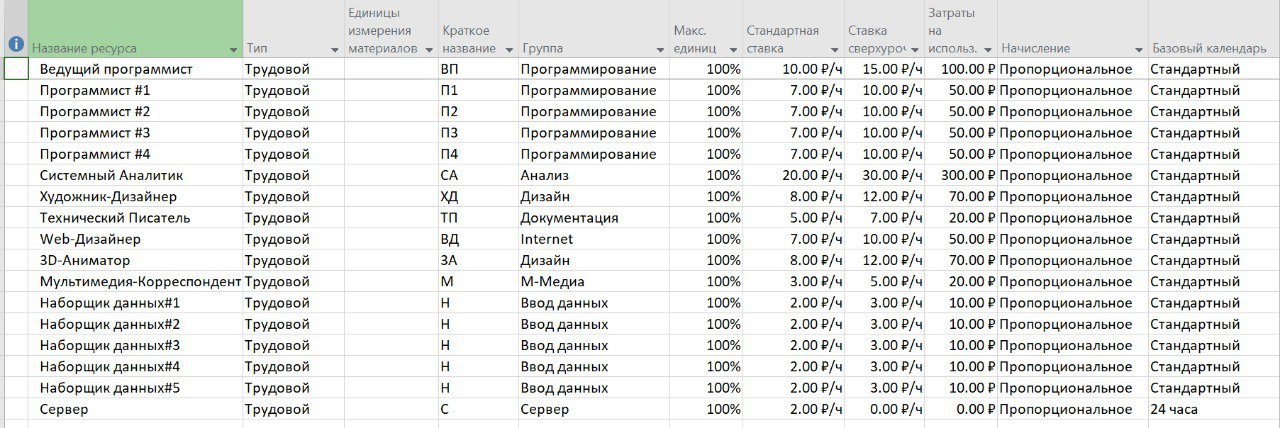
\includegraphics[width=\linewidth]{inc/1-2.jpeg}
	\end{center}
	\captionsetup{justification=centering}
	\caption{Текущая загрузка ресурсов}
\end{figure}
\FloatBarrier 

\newpage
\anonsection{Задание 2}
В этом задании нужно учесть периодические задачи в плане проекта.

\subsection*{Добавление еженедельного совещания}
В плане требуется отразить организацию еженедельного совещания по средам с 10 до 11 часов.

Для этого использовался подпункт меню \textit{Задача} -> \textit{Добавить новую повторяющуюся задачу}.
На рисунке 3 представлено меню добавления новой повторяющейся задачи:
\FloatBarrier
\begin{figure}[h]	
	\begin{center}
		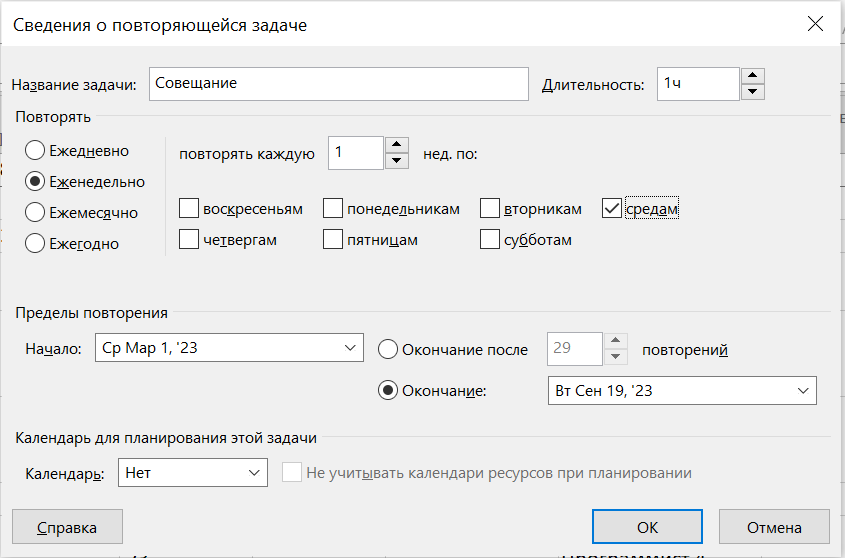
\includegraphics[width=\linewidth]{inc/rep.png}
	\end{center}
	\captionsetup{justification=centering}
	\caption{Добавление еженедельного совещания}
\end{figure}
\FloatBarrier 

В качестве использованных на собрании людей выбраны следующие специалисты:
\FloatBarrier
\begin{figure}[h]	
	\begin{center}
		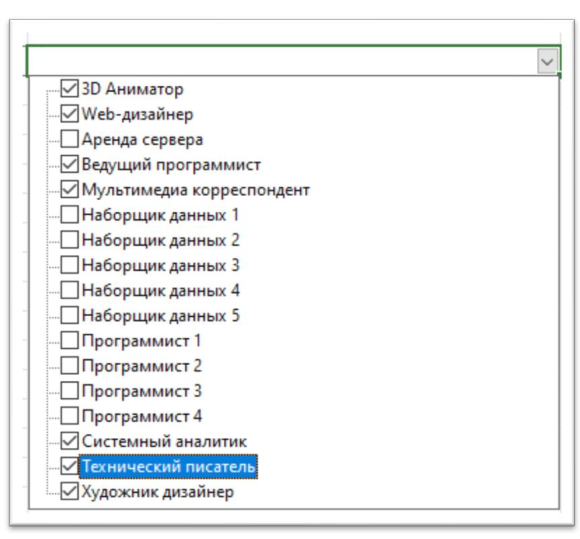
\includegraphics[width=\linewidth]{inc/2-2.png}
	\end{center}
	\captionsetup{justification=centering}
	\caption{Добавленные к задачам ресурсы}
\end{figure}
\FloatBarrier 

\subsection*{Устранение перегрузки ресурсов}
Из-за добавления совещаний каждый специалист из участвующих в собрании оказался перегружен.

\FloatBarrier
\begin{figure}[h]	
	\begin{center}
		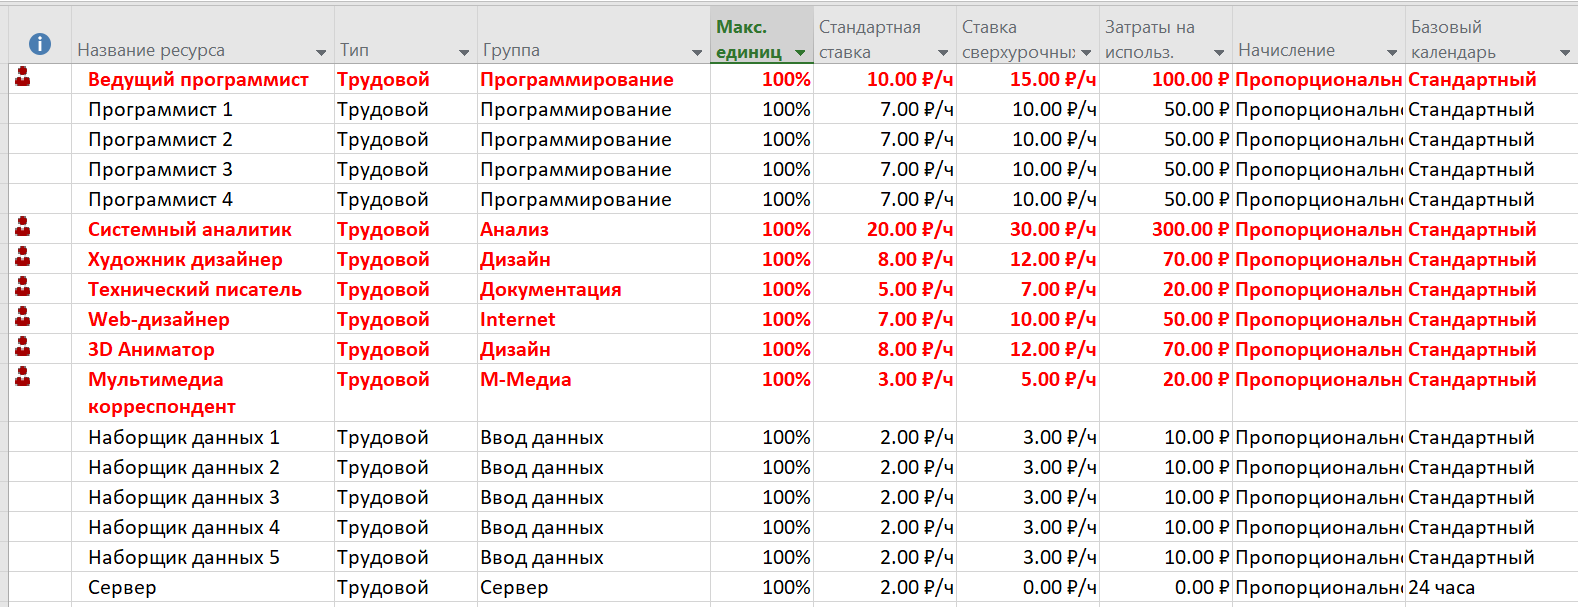
\includegraphics[width=\linewidth]{inc/list.png}
	\end{center}
	\captionsetup{justification=centering}
	\caption{Перегрузка ресурсов}
\end{figure}
\FloatBarrier 

Для исправлений перегрузки ресурсов были применены следующие меры:
\begin{itemize}
	\item использована аналогичная заданию 1 перегрузка ресурсов.
	\item на одном из собраний не будет присутствовать Web-дизайнер, так как интересы его задачи будет представлять Художник-Дизайнер.
\end{itemize}

В итоге перегрузка ресурсов была устранена, что видно на рисунке 6:
\FloatBarrier
\begin{figure}[h]	
	\begin{center}
		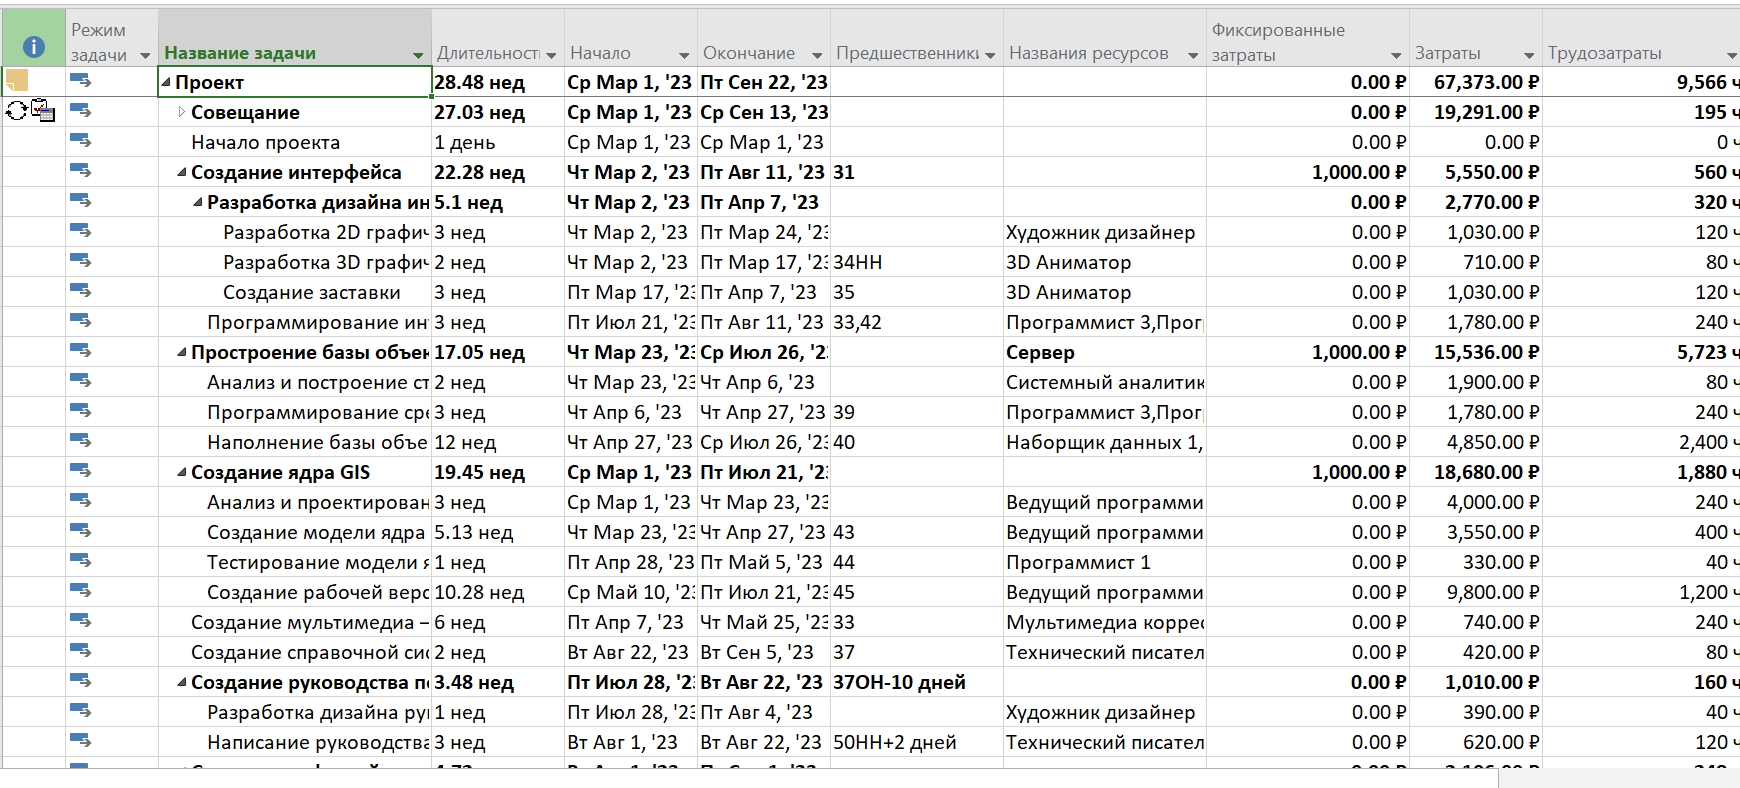
\includegraphics[width=\linewidth]{inc/after.png}
	\end{center}
	\captionsetup{justification=centering}
	\caption{Устранение перегрузки ресурсов}
\end{figure}
\FloatBarrier 

Сроки проекта сдвинулись до 22 сентября.

\subsection*{Анализ и оптимизация бюджета}
На текущем этапе у проекта выявлены следующие проблемы:
\begin{enumerate}
	\item Проект не успевает к заявленным срокам -- требуется закончить работу до 1 сентября, а сейчас конечная дата -- 22 сентября.
	\item Ожидаемый расход составляет 67373 рубля, в то время как бюджет организации -- лишь 50000 рублей. 
	Проблема возникла из-за появления еженедельных собраний, который входит в рабочий день.
\end{enumerate}

Для того, чтобы решить вторую проблему, достаточно не платить работникам за совещания, так как в ходе её деятельности работники не занимаются непосредственно проектом.
Это можно сделать в пункте \textit{Вид} -> \textit{Использование ресурсов}. 
У всех работников для задач совещания стоит режим затрат по-умолчанию, но можно изменить режим на B со стандартной ставкой 0 руб.

\newpage
\anonsection{Задание 3}
В этом задании требуется оптимизировать критический путь и сократить его на две недели.

Самые продолжительные задачи для программистов -- это создание рабочей версии ядра и программирование интерфейсов.
Они могут выполняться последовательно, поэтому для их решения может быть подключена вся команда.

Чтобы успеть по срокам, были приняты следующие меры:
\begin{enumerate}
	\item Для программирования интерфейсов и создания рабочей версии ядра были использованы все программисты, а не только два. Это возможно, так как задачи не пересекаются друг с другом.
	\item Все лишние совещания удалены.
\end{enumerate}

Дедлайн по проекту сдвинулся до 16 августа, а расходы составили 48299 рублей.

На рисунке 7 изображен итоговый результат:
\FloatBarrier
\begin{figure}[h]	
	\begin{center}
		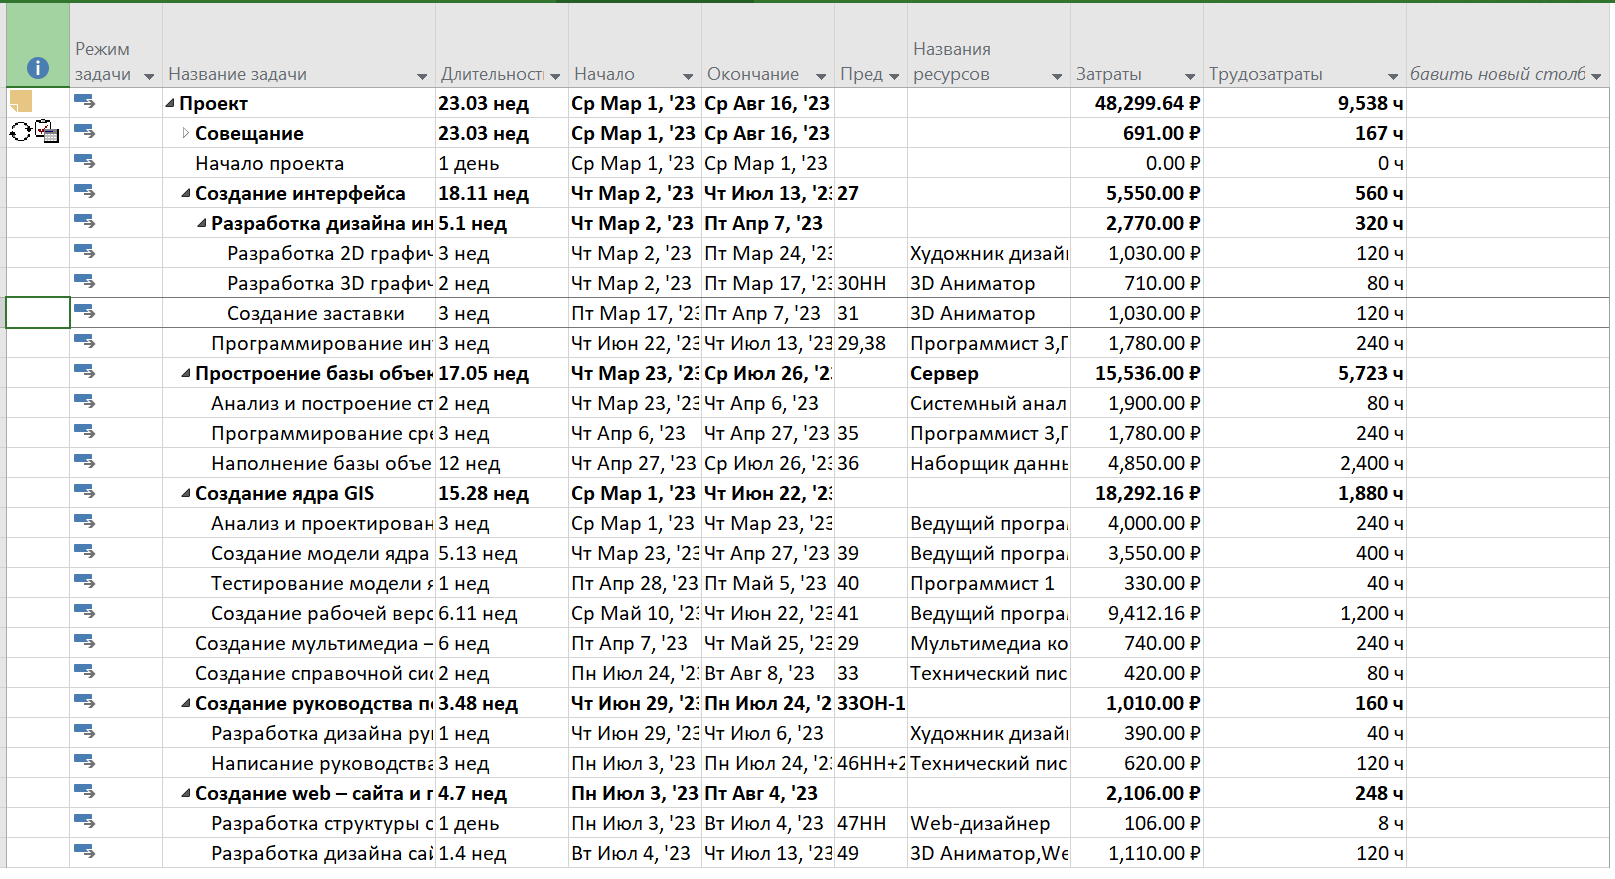
\includegraphics[width=\linewidth]{inc/result.png}
	\end{center}
	\captionsetup{justification=centering}
	\caption{Результат оптимизации критического пути и бюджета}
\end{figure}
\FloatBarrier 

Соотношение затрат и трудозатрат существенно не изменилось по сравнению с прошлой лабораторной работой.

Графики абсолютных и относительных величин затрат и трудозатрат представлены на рисунках 8 и 9:
\FloatBarrier
\begin{figure}[h]	
	\begin{center}
		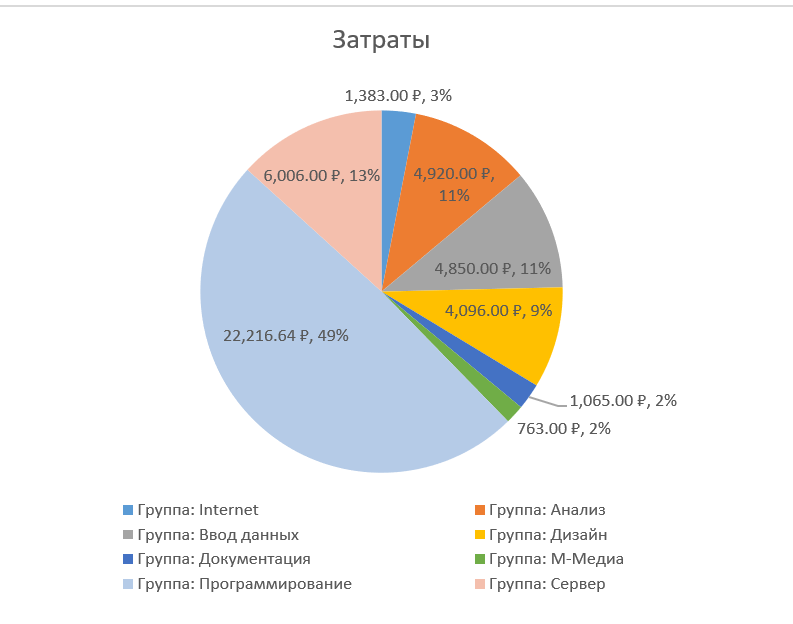
\includegraphics[width=\linewidth]{inc/zp.png}
	\end{center}
	\captionsetup{justification=centering}
	\caption{Затраты в проекте}
\end{figure}
\FloatBarrier 

\FloatBarrier
\begin{figure}[h]	
	\begin{center}
		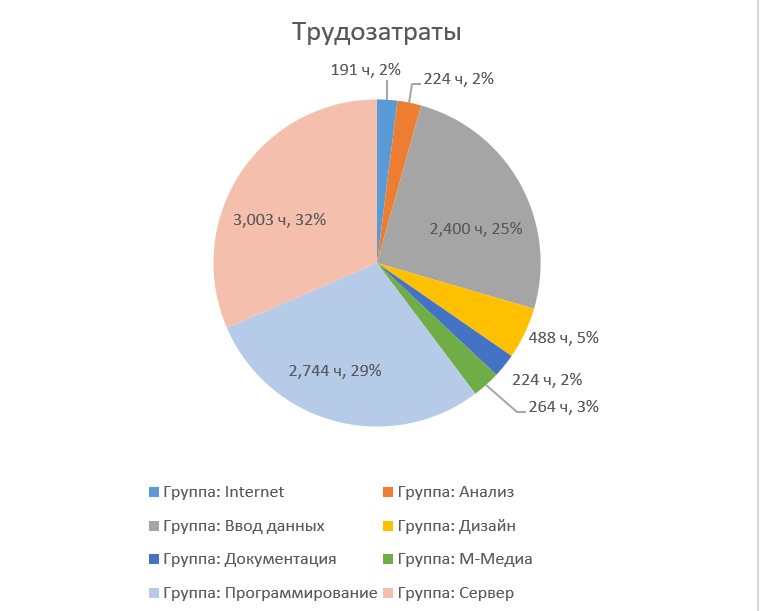
\includegraphics[width=\linewidth]{inc/trud.png}
	\end{center}
	\captionsetup{justification=centering}
	\caption{Трудозатраты в проекте}
\end{figure}
\FloatBarrier 

\newpage
Создание базового плана проекта было выполнено в подменю \textit{Проект} -> \textit{Создание базового плана проекта}.
Меню представлено на рисунке 10:
\FloatBarrier
\begin{figure}[h]	
	\begin{center}
		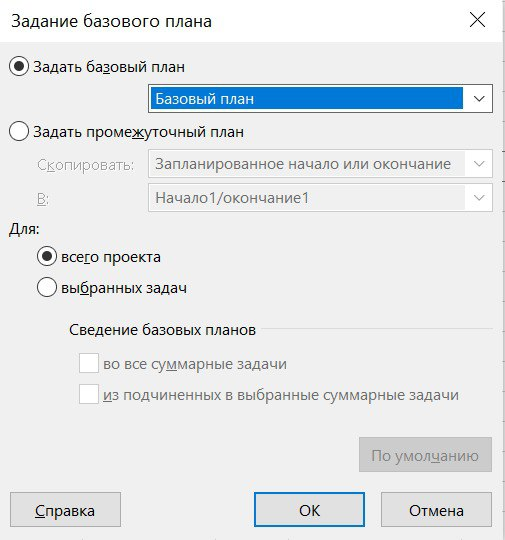
\includegraphics[width=\linewidth]{inc/4-4.jpeg}
	\end{center}
	\captionsetup{justification=centering}
	\caption{Создание базового плана проекта}
\end{figure}
\FloatBarrier 

\anonsection{Выводы}
В результате выполнения лабораторной работы был составлен базовый план проекта.

Теперь сроки выполнения проекта составляют 5.5 месяцев, то есть оптимизации позволили уменьшить время реализации на 1 месяц.
В результате добавления еженедельных совещаний был превышен бюджет, но с помощью изменения режима оплаты дефицит был ликвидирован.
Перегрузок по ресурсам в проекте нет.

Из возможностей Microsoft Project были использованы \textbf{Автоматическое выравнивание ресурсов проекта} и \textbf{Добавление новой повторяющейся задачи}.